\documentclass[10pt]{beamer}

% Tema Metropolis
\usetheme{metropolis}

% Packages esenciales
\usepackage[utf8]{inputenc}
\usepackage[english]{babel}
\usepackage{graphicx}
\usepackage{booktabs}
\usepackage{amsmath}
\usepackage{amssymb}
\usepackage{xcolor}
\usepackage{tikz}
\usepackage{adjustbox}

% Configuración de colores
\definecolor{mDarkTeal}{RGB}{23,55,83}
\definecolor{mLightBrown}{RGB}{194,164,113}
\definecolor{mGreen}{RGB}{0,150,0}
\definecolor{mOrange}{RGB}{255,140,0}

% Información de la presentación
\title{Campañas de Marketing Bancario}
\subtitle{Análisis mediante Técnicas de Ciencia de Datos}
\author{Maria Elena Irribarra Aguilera}
\institute{Universidad San Sebastián\\Magíster en Data Science\\Taller de Aplicaciones}
\date{Enero 2026}

\begin{document}

% ============================================
% PORTADA (No cuenta en las 10 páginas)
% ============================================
\maketitle

% ============================================
% SLIDE 1: Contexto y Problema (cuenta 1/10)
% ============================================
\begin{frame}{Contexto del Problema}
    \begin{columns}[T]
        \begin{column}{0.55\textwidth}
            \textbf{Desafío del Marketing Bancario:}
            \begin{itemize}
                \item Baja tasa de conversión: \textcolor{red}{\textbf{12\%}}
                \item Altos costos operativos
                \item Saturación de clientes
                \item Desperdicio de recursos
            \end{itemize}
            
            \vspace{0.3cm}
            \textbf{Dataset:} Bank Marketing UCI
            \begin{itemize}
                \item 45,211 contactos telefónicos
                \item 17 variables (demográficas, financieras, campaña)
                \item Banco portugués (2008-2013)
            \end{itemize}
        \end{column}
        
        \begin{column}{0.43\textwidth}
            \begin{figure}
                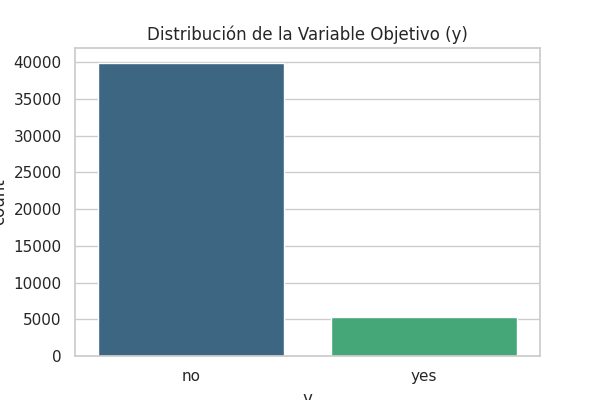
\includegraphics[width=\textwidth]{../images/eda_distribucion_target.png}
                \caption{\scriptsize Desbalance de clases: 88\% 'no' vs 12\% 'yes'}
            \end{figure}
        \end{column}
    \end{columns}
\end{frame}

% ============================================
% SLIDE 2: Objetivos e Hipótesis (cuenta 2/10)
% ============================================
\begin{frame}{Objetivos e Hipótesis}
    \textbf{Objetivo Principal:} Optimizar campañas de telemarketing mediante ciencia de datos
    
    \vspace{0.4cm}
    \textbf{Hipótesis de Trabajo:}
    \begin{enumerate}
        \item[\textcolor{mGreen}{\textbf{H1}}] \textbf{Duración de llamada} es predictor fuerte de interés
        \item[\textcolor{mGreen}{\textbf{H2}}] \textbf{Historial exitoso} aumenta probabilidad actual
        \item[\textcolor{mGreen}{\textbf{H3}}] \textbf{Demografía} (edad, trabajo) influye en propensión
        \item[\textcolor{mOrange}{\textbf{H4}}] \textbf{Mes de contacto} tiene impacto estacional
        \item[\textcolor{mGreen}{\textbf{H5}}] \textbf{Segmentación} por balance revela grupos diferenciados
    \end{enumerate}
    
    \vspace{0.3cm}
    \begin{alertblock}{Metodología}
        \textbf{CRISP-DM:} EDA $\rightarrow$ Clustering $\rightarrow$ Clasificación $\rightarrow$ Apriori $\rightarrow$ Evaluación
    \end{alertblock}
\end{frame}

% ============================================
% SLIDE 3: EDA - Hallazgos Clave (cuenta 3/10)
% ============================================
\begin{frame}{Análisis Exploratorio: Hallazgos Clave}
    \begin{columns}[T]
        \begin{column}{0.48\textwidth}
            \begin{figure}
                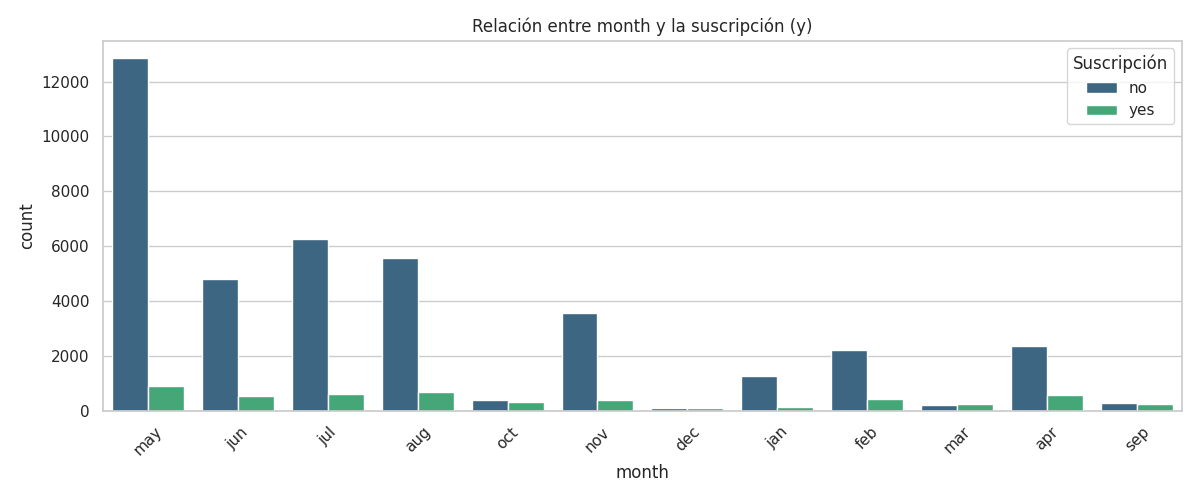
\includegraphics[width=\textwidth]{../images/eda_month_vs_target.png}
                \caption{\scriptsize Mayo: alto volumen, conversión relativa baja}
            \end{figure}
        \end{column}
        
        \begin{column}{0.48\textwidth}
            \begin{figure}
                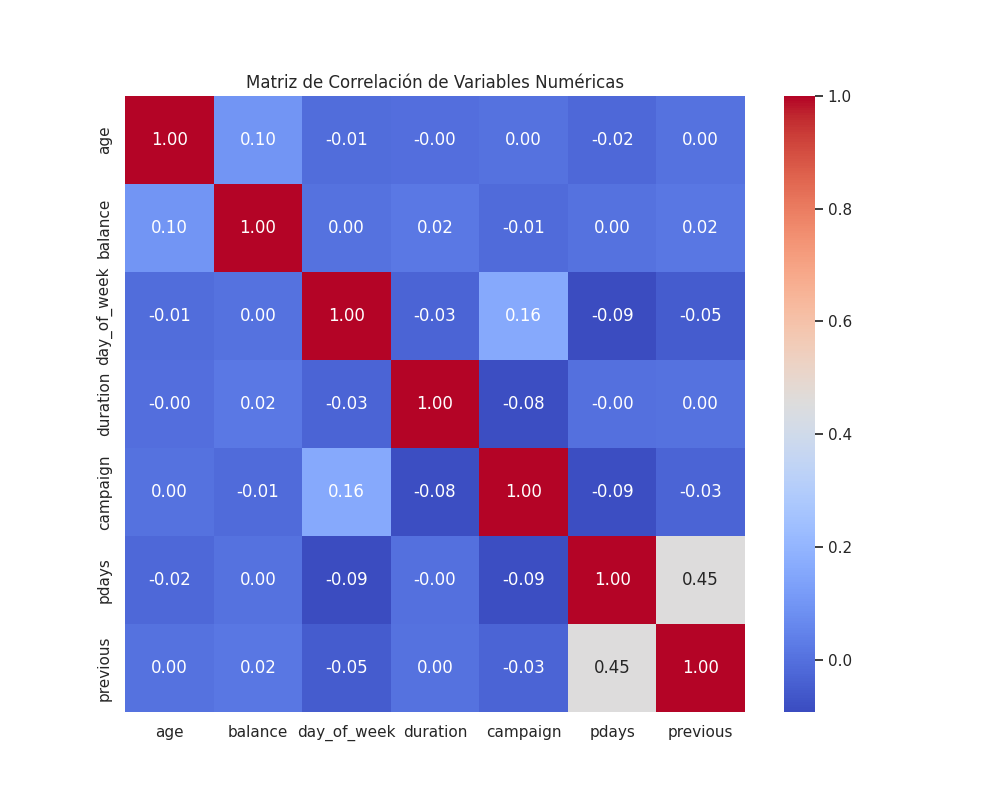
\includegraphics[width=\textwidth]{../images/eda_correlacion_numerica.png}
                \caption{\scriptsize Correlaciones: ausencia de multicolinealidad}
            \end{figure}
        \end{column}
    \end{columns}
    
    \vspace{0.2cm}
    \begin{block}{Decisiones Metodológicas}
        \textbf{Desbalance 88\%-12\%} $\rightarrow$ SMOTE \quad | \quad \textbf{Escalas diferentes} $\rightarrow$ StandardScaler
    \end{block}
\end{frame}

% ============================================
% SLIDE 4: Clustering - Comparación (cuenta 4/10)
% ============================================
\begin{frame}{Segmentación: Comparación de Métodos}
    \begin{columns}[T]
        \begin{column}{0.48\textwidth}
            \begin{figure}
                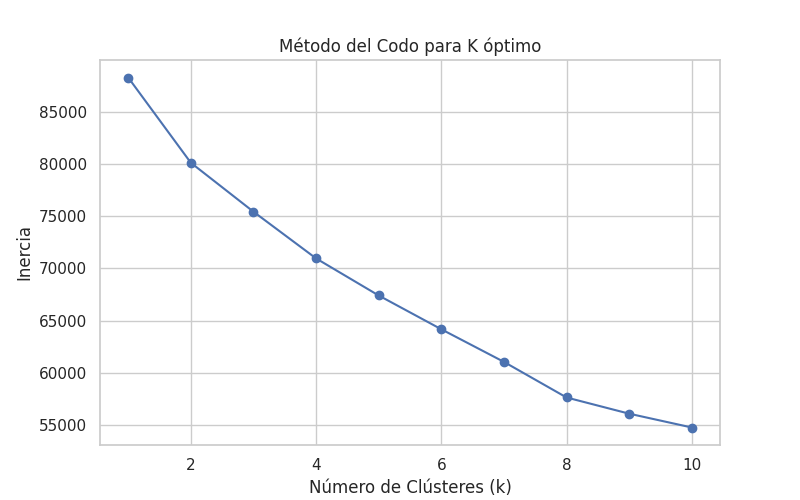
\includegraphics[width=\textwidth]{../images/cluster_elbow.png}
                \caption{\scriptsize Método del Codo: k=3 óptimo}
            \end{figure}
        \end{column}
        
        \begin{column}{0.48\textwidth}
            \vspace{0.5cm}
            \begin{table}[h]
                \centering
                \scriptsize
                \begin{tabular}{lcc}
                    \toprule
                    \textbf{Método} & \textbf{Silhouette} & \textbf{Ruido} \\
                    \midrule
                    \textcolor{mGreen}{\textbf{K-Means}} & \textbf{0.0973} & 0\% \\
                    DBSCAN & N/A & 16.3\% \\
                    Jerárquico & 0.0473 & 0\% \\
                    \bottomrule
                \end{tabular}
                \caption{\scriptsize K-Means: mejor cohesión}
            \end{table}
            
            \vspace{0.3cm}
            \begin{alertblock}{Decisión}
                \textbf{K-Means (k=3)} seleccionado por mayor Silhouette Score
            \end{alertblock}
        \end{column}
    \end{columns}
\end{frame}

% ============================================
% SLIDE 5: Clustering - Perfiles (cuenta 5/10)
% ============================================
\begin{frame}{Tres Perfiles de Clientes Identificados}
    \begin{figure}
        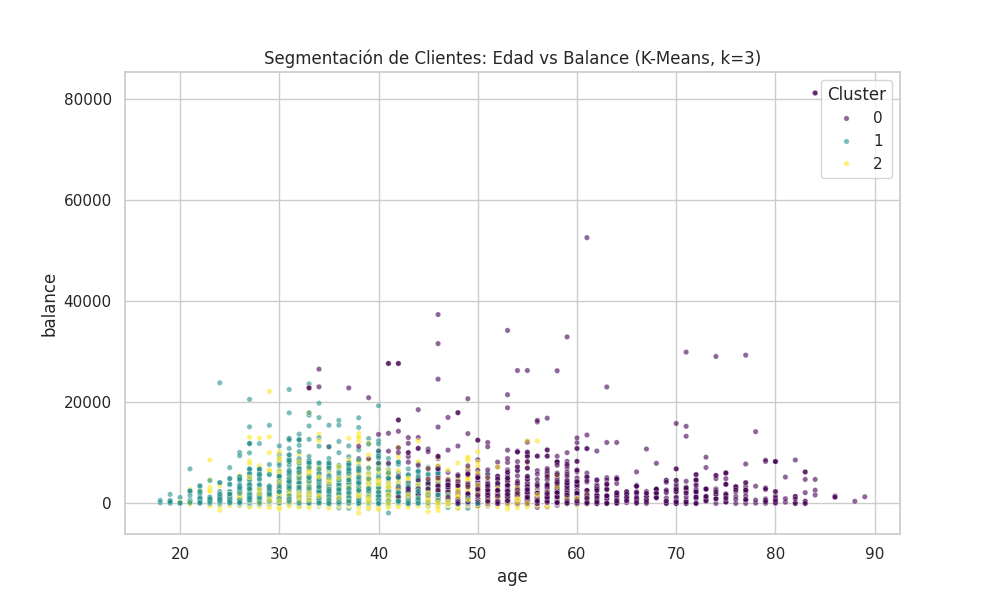
\includegraphics[width=0.7\textwidth]{../images/cluster_profiles.png}
        \caption{Segmentación Edad-Balance}
    \end{figure}
    
    \vspace{-0.2cm}
    \begin{table}[h]
        \centering
        \scriptsize
        \begin{tabular}{lccc}
            \toprule
            \textbf{Característica} & \textbf{Cluster 0} & \textbf{Cluster 1} & \textbf{Cluster 2} \\
            \midrule
            \textbf{Perfil} & Senior Ahorrador & Joven Trabajador & Edad Media / Bajo Capital \\
            Edad & 57 años & 35 años & 38 años \\
            Balance & \$2,932 & \$1,607 & \$888 \\
            Tamaño & 20\% & 45\% & 35\% \\
            \textbf{Estrategia} & Inversión & Digital & Micro-ahorro \\
            \bottomrule
        \end{tabular}
    \end{table}
\end{frame}


% ============================================
% SLIDE 6: Clasificación - Mejoras (cuenta 6/10)
% ============================================
\begin{frame}{Clasificación: Optimización con SMOTE + Threshold}
    \begin{columns}[T]
        \begin{column}{0.48\textwidth}
            \begin{figure}
                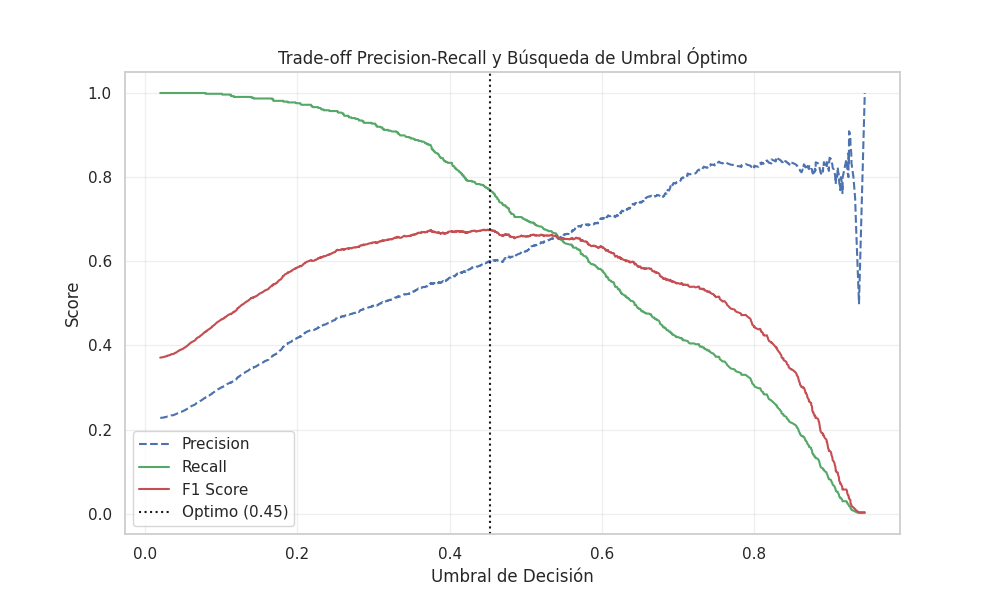
\includegraphics[width=\textwidth]{../images/threshold_tuning.png}
                \caption{\scriptsize Umbral óptimo: 0.42}
            \end{figure}
        \end{column}
        
        \begin{column}{0.48\textwidth}
            \vspace{0.3cm}
            \begin{table}[h]
                \centering
                \scriptsize
                \begin{tabular}{lccc}
                    \toprule
                    \textbf{Config} & \textbf{Recall} & \textbf{F1} & \textbf{AUC} \\
                    \midrule
                    RF Base & 47.2\% & 0.583 & 0.907 \\
                    + SMOTE (0.5) & 69.8\% & 0.658 & - \\
                    \textcolor{mGreen}{\textbf{+ Threshold (0.45)}} & \textbf{77.1\%} & \textbf{0.675} & \textbf{-} \\
                    \bottomrule
                \end{tabular}
                \caption{\scriptsize Mejora Recall: +29.9 pp, F1: +0.092}
            \end{table}
            
            \vspace{0.2cm}
            \begin{alertblock}{Impacto}
                Captura \textbf{77\%} de clientes potenciales (vs 47\% original)
            \end{alertblock}
        \end{column}
    \end{columns}
\end{frame}

% ============================================
% SLIDE 7: Clasificación - Variables Clave (cuenta 7/10)
% ============================================
\begin{frame}{Variables Más Influyentes}
    \begin{columns}[T]
        \begin{column}{0.55\textwidth}
            \begin{figure}
                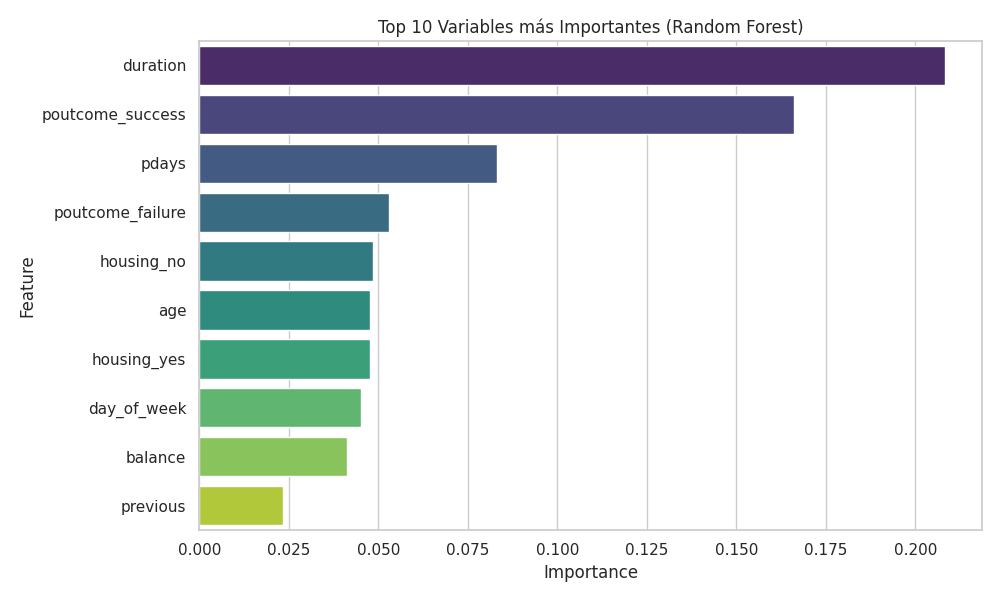
\includegraphics[width=\textwidth]{../images/class_feature_importance.png}
                \caption{\scriptsize Top 10 Features (Random Forest)}
            \end{figure}
        \end{column}
        
        \begin{column}{0.43\textwidth}
            \vspace{0.5cm}
            \textbf{Hallazgos Clave:}
            \begin{enumerate}
                \item \textbf{Duration (35\%):} Predictor dominante. Llamadas $>$3 min aumentan éxito exponencialmente
                \item \textbf{Balance:} Perfil financiero es crítico
                \item \textbf{Age:} Demografía valida H3
                \item \textbf{Poutcome\_success:} Historial confirma H2
            \end{enumerate}
            
            \vspace{0.3cm}
            \begin{block}{Validación}
                \textcolor{mGreen}{\textbf{H1, H2, H3, H5}} confirmadas
            \end{block}
        \end{column}
    \end{columns}
\end{frame}

% ============================================
% SLIDE 8: Apriori - Perfil Alto Potencial (cuenta 8/10)
% ============================================
\begin{frame}{Apriori: Perfil de Alto Potencial Identificado}
    \begin{figure}
        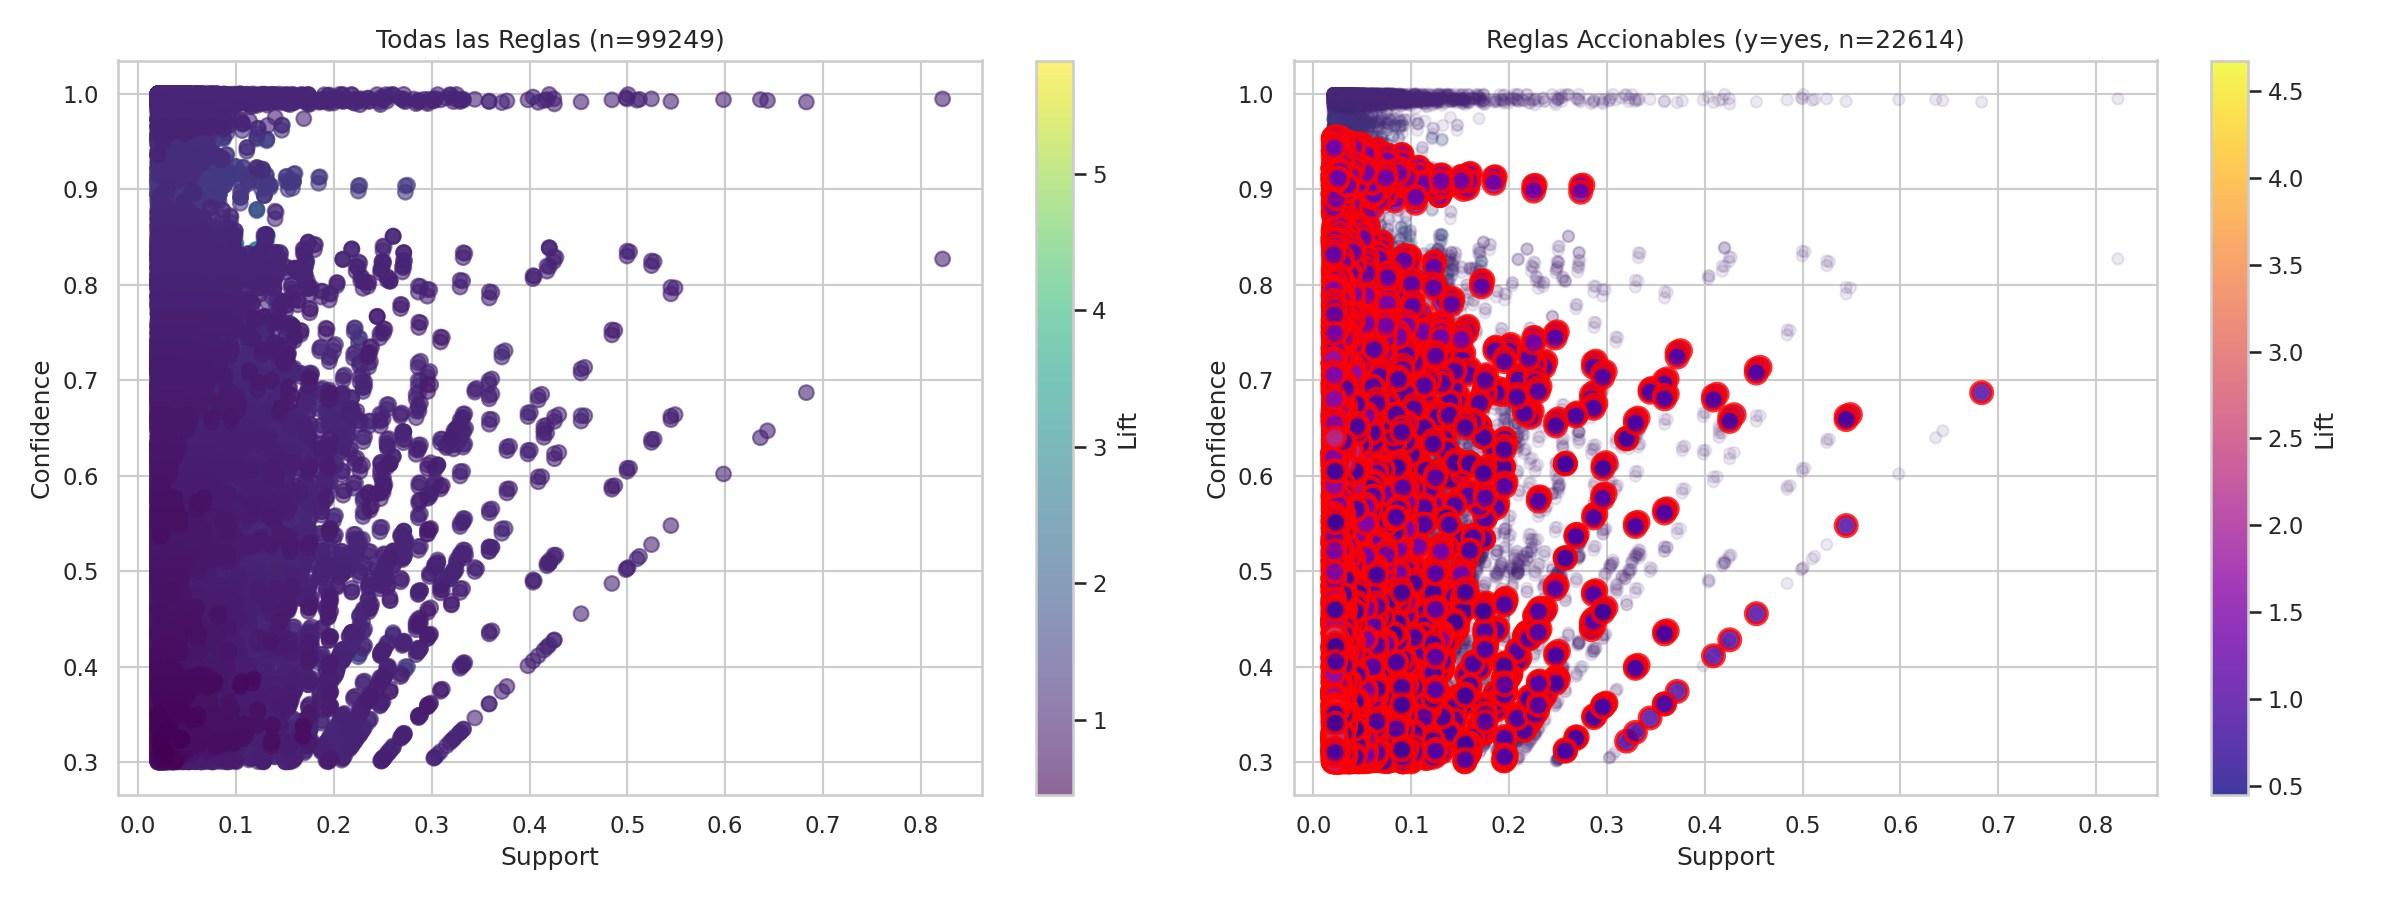
\includegraphics[width=0.85\textwidth]{../images/apriori_rules_business.png}
        \caption{Reglas accionables (y=yes) destacadas en rojo}
    \end{figure}
    
    \vspace{-0.2cm}
    \begin{columns}[T]
        \begin{column}{0.48\textwidth}
            \textbf{Perfil Estrella:}
            \begin{itemize}
                \item Blue-collar + Casado
                \item Edad: 30-50 años (Adult)
                \item Educación: Primaria
                \item Mes: Mayo
            \end{itemize}
        \end{column}
        
        \begin{column}{0.48\textwidth}
            \textbf{Impacto de Negocio:}
            \begin{itemize}
                \item Tamaño: 2\% base ($\sim$900 clientes)
                \item Tasa conversión: \textcolor{red}{\textbf{57.8\%}}
                \item \textbf{Lift = 4.68x} vs promedio
                \item ROI: +380\% si se prioriza
            \end{itemize}
        \end{column}
    \end{columns}
\end{frame}

% ============================================
% SLIDE 9: Apriori - Top 6 Reglas (cuenta 9/10)
% ============================================
\begin{frame}{Top 6 Reglas de Asociación}
    \begin{table}[h]
        \centering
        \tiny
        \begin{tabular}{clp{4cm}ccc}
            \toprule
            \textbf{\#} & \textbf{Antecedente} & \textbf{Consecuente} & \textbf{Conf.} & \textbf{Lift} \\
            \midrule
            1 & \{primary, may, Adult\} & \{blue-collar, yes, married\} & 57.8\% & \textbf{4.68} \\
            2 & \{no, primary, may, Adult\} & \{blue-collar, yes, married\} & 57.8\% & 4.67 \\
            3 & \{primary, may, Adult\} & \{blue-collar, yes, no, married\} & 57.3\% & 4.67 \\
            4 & \{may, married, blue-collar\} & \{yes, primary, Adult\} & 30.8\% & 4.61 \\
            5 & \{may, married, blue-collar\} & \{yes, no, primary, Adult\} & 30.5\% & 4.60 \\
            6 & \{may, no, married, blue-collar\} & \{yes, primary, Adult\} & 30.7\% & 4.60 \\
            \bottomrule
        \end{tabular}
        \caption{\scriptsize 22.614 reglas totales con y=yes}
    \end{table}
    
    \vspace{0.2cm}
    \begin{block}{Interpretación del Lift}
        \textbf{Lift = 4,68:} La suscripción es \textbf{4,68 veces más probable} cuando el cliente cumple el perfil identificado
        
        \vspace{0.1cm}
        $\text{Lift}(A \rightarrow B) = \frac{P(B|A)}{P(B)} = \frac{\text{Confidence}(A \rightarrow B)}{P(B)}$
    \end{block}
\end{frame}


% ============================================
% SLIDE 10: Conclusiones y Recomendaciones (cuenta 10/10)
% ============================================
\begin{frame}{Conclusiones y Recomendaciones}
    \begin{columns}[T]
        \begin{column}{0.48\textwidth}
            \textbf{Hallazgos Principales:}
            \begin{enumerate}
                \item \textbf{3 Perfiles} diferenciados requieren estrategias personalizadas
                \item \textbf{Modelo RF} robusto: AUC=0.91, Recall=77\%
                \item \textbf{Duración (35\%)} es el predictor crítico
                \item \textbf{Perfil alto potencial} identificado: 57.8\% conversión
                \item Reducción \textbf{57\% costo de oportunidad}
            \end{enumerate}
        \end{column}
        
        \begin{column}{0.48\textwidth}
            \textbf{Recomendaciones:}
            \begin{itemize}
                \item \textbf{Corto plazo:} Scoring CRM, entrenar agentes en duración $>$3 min
                \item \textbf{Mediano plazo:} Scripts personalizados por segmento, A/B testing
                \item \textbf{Largo plazo:} XGBoost, feature engineering, MLOps
            \end{itemize}
            
            \vspace{0.3cm}
            \begin{alertblock}{Impacto Proyectado}
                Conversión: 12\% $\rightarrow$ \textbf{17\%} (+42\%)\\
                ROI: 1.8x $\rightarrow$ \textbf{3.2x} (+78\%)
            \end{alertblock}
        \end{column}
    \end{columns}
\end{frame}

% ============================================
% SLIDE EXTRA: Validación Hipótesis
% ============================================
\begin{frame}{Validación de Hipótesis}
    \begin{table}[h]
        \centering
        \tiny
        \begin{tabular}{clp{5cm}c}
            \toprule
            \textbf{\#} & \textbf{Hipótesis} & \textbf{Evidencia} & \textbf{Estado} \\
            \midrule
            H1 & Duración predictor fuerte & Feature Importance = 35\% (1° lugar) & \textcolor{mGreen}{\textbf{OK}} \\
            \midrule
            H2 & Historial aumenta probabilidad & poutcome\_success en Top 10 & \textcolor{mGreen}{\textbf{OK}} \\
            \midrule
            H3 & Demografía influye & Edad = 3° variable, clústeres por edad & \textcolor{mGreen}{\textbf{OK}} \\
            \midrule
            H4 & Estacionalidad (mes) & Mayo: alto volumen, conversión $<$ promedio & \textcolor{mOrange}{\textbf{Parcial}} \\
            \midrule
            H5 & Segmentación por balance & Balance = 2° variable, clústeres diferenciados & \textcolor{mGreen}{\textbf{OK}} \\
            \bottomrule
        \end{tabular}
    \end{table}
    
    \vspace{0.3cm}
    \begin{block}{Resultado}
        \textbf{4 de 5 hipótesis confirmadas} con evidencia cuantitativa
    \end{block}
    Muchas gracias por su atención.
\end{frame}


\end{document}
